\documentclass[12pt, titlepage]{article}

\usepackage{fullpage}
\usepackage[round]{natbib}
\usepackage{multirow}
\usepackage{booktabs}
\usepackage{tabularx}
\usepackage{graphicx}
\usepackage{float}
\usepackage{hyperref}
\hypersetup{
    colorlinks,
    citecolor=blue,
    filecolor=black,
    linkcolor=red,
    urlcolor=blue
}

%% Comments

\usepackage{color}

\newif\ifcomments\commentstrue %displays comments
%\newif\ifcomments\commentsfalse %so that comments do not display

\ifcomments
\newcommand{\authornote}[3]{\textcolor{#1}{[#3 ---#2]}}
\newcommand{\todo}[1]{\textcolor{red}{[TODO: #1]}}
\else
\newcommand{\authornote}[3]{}
\newcommand{\todo}[1]{}
\fi

\newcommand{\wss}[1]{\authornote{blue}{SS}{#1}} 
\newcommand{\plt}[1]{\authornote{magenta}{TPLT}{#1}} %For explanation of the template
\newcommand{\an}[1]{\authornote{cyan}{Author}{#1}}

%% Common Parts

\newcommand{\progname}{Flick Picker}
\newcommand{\authname}{Team 7, 7eam
\\ Talha Asif - asift
\\ Jarrod Colwell - colwellj
\\ Madhi Nagarajan - nagarajm
\\ Andrew Carvalino - carvalia    
\\ Ali Tabar - sahraeia
}     

\usepackage{hyperref}
    \hypersetup{colorlinks=true, linkcolor=blue, citecolor=blue, filecolor=blue,
                urlcolor=blue, unicode=false}
    \urlstyle{same}
                                


\newcounter{acnum}
\newcommand{\actheacnum}{AC\theacnum}
\newcommand{\acref}[1]{AC\ref{#1}}

\newcounter{ucnum}
\newcommand{\uctheucnum}{UC\theucnum}
\newcommand{\uref}[1]{UC\ref{#1}}

\newcounter{mnum}
\newcommand{\mthemnum}{M\themnum}
\newcommand{\mref}[1]{M\ref{#1}}

\begin{document}

\title{Module Guide for \progname{}} 
\author{\authname}
\date{\today}

\maketitle

\pagenumbering{roman}

\section{Revision History}

\begin{tabularx}{\textwidth}{p{3cm}p{2cm}X}
\toprule {\bf Date} & {\bf Version} & {\bf Notes}\\
\midrule
Jan 14 & 0.1 & Adding modules and objects to store in databases - Talha\\
Jan 15 & 0.1 & Adding descriptions to modules - Talha\\
April 5 & 1.0 & Updated Custom Data Types, minor changes - Madhi \\
April 5 & 1.1 & Added links to relevant documents - Ali \\
\bottomrule
\end{tabularx}

\newpage

\section{Reference Material}

Complementary documents include the Module Interface Specification and the System Requirement Specifications.
The full documentation and implementation can be
found at \url{https://github.com/Flick-Picker/full-stack}.

See Module Interface Specification at \url{https://github.com/Flick-Picker/full-stack/blob/develop/docs/Design/SoftDetailedDes/MIS.pdf}.
See System Requirement Specifications at \url{https://github.com/Flick-Picker/full-stack/blob/develop/docs/SRS/SRS.pdf}.

\subsection{Abbreviations and Acronyms}

\renewcommand{\arraystretch}{1.2}
\begin{tabular}{l l} 
  \toprule		
  \textbf{symbol} & \textbf{description}\\
  \midrule 
  AC & Anticipated Change\\
  DAG & Directed Acyclic Graph \\
  M & Module \\
  MG & Module Guide \\
  OS & Operating System \\
  R & Requirement\\
  SC & Scientific Computing \\
  SRS & Software Requirements Specification\\
  \progname & Application\\
  UC & Unlikely Change \\
  \bottomrule
\end{tabular}\\

\newpage

\tableofcontents

\listoftables

\listoffigures

\newpage

\pagenumbering{arabic}

\section{Introduction}

Decomposing a system into modules is a commonly accepted approach to developing
software.  A module is a work assignment for a programmer or programming
team~\citep{ParnasEtAl1984}.  We advocate a decomposition
based on the principle of information hiding~\citep{Parnas1972a}.  This
principle supports design for change, because the ``secrets'' that each module
hides represent likely future changes.  Design for change is valuable in SC,
where modifications are frequent, especially during initial development as the
solution space is explored.  

Our design follows the rules layed out by \citet{ParnasEtAl1984}, as follows:
\begin{itemize}
\item System details that are likely to change independently should be the
  secrets of separate modules.
\item Each data structure is implemented in only one module.
\item Any other program that requires information stored in a module's data
  structures must obtain it by calling access programs belonging to that module.
\end{itemize}

After completing the first stage of the design, the Software Requirements
Specification (SRS), the Module Guide (MG) is developed~\citep{ParnasEtAl1984}. The MG
specifies the modular structure of the system and is intended to allow both
designers and maintainers to easily identify the parts of the software.  The
potential readers of this document are as follows:

\begin{itemize}
\item New Project Members: This document can be a guide for a new project member
  to easily understand the overall structure and quickly find the
  relevant modules they are searching for.
\item Maintainers: The hierarchical structure of the module guide improves the
  maintainers' understanding when they need to make changes to the system. It is
  important for a maintainer to update the relevant sections of the document
  after changes have been made.
\item Designers: Once the module guide has been written, it can be used to
  check for consistency, feasibility, and flexibility. Designers can verify the
  system in various ways, such as consistency among modules, feasibility of the
  decomposition, and flexibility of the design.
\end{itemize}

The rest of the document is organized as follows. Section
\ref{SecChange} lists the anticipated and unlikely changes of the software
requirements. Section \ref{SecMH} summarizes the module decomposition that
was constructed according to the likely changes. Section \ref{SecConnection}
specifies the connections between the software requirements and the
modules. Section \ref{SecCD} provides detailed descriptions of native data types. Section \ref{SecMD} gives a detailed description of the
modules. Section \ref{SecTM} includes two traceability matrices. One checks
the completeness of the design against the requirements provided in the SRS. The
other shows the relation between anticipated changes and the modules. Section
\ref{SecUse} describes the use relation between modules.

\section{Anticipated and Unlikely Changes} \label{SecChange}

This section lists possible changes to the system. According to the likeliness
of the change, the possible changes are classified into two
categories. Anticipated changes are listed in Section \ref{SecAchange}, and
unlikely changes are listed in Section \ref{SecUchange}.

\subsection{Anticipated Changes} \label{SecAchange}

Anticipated changes are the source of the information that is to be hidden
inside the modules. Ideally, changing one of the anticipated changes will only
require changing the one module that hides the associated decision. The approach
adapted here is called design for
change.

\begin{description}
\item[\refstepcounter{acnum} \actheacnum \label{acHardware}:] The specific hardware on which the software is running.
\item[\refstepcounter{acnum} \actheacnum \label{acPrefs}:] The \verb_preferences_ could be modified, depending on what the general response to the initial show preferences exist
\end{description}

\subsection{Unlikely Changes} \label{SecUchange}

The module design should be as general as possible. However, a general system is
more complex. Sometimes this complexity is not necessary. Fixing some design
decisions at the system architecture stage can simplify the software design. If
these decision should later need to be changed, then many parts of the design
will potentially need to be modified. Hence, it is not intended that these
decisions will be changed.

\begin{description}
\item[\refstepcounter{ucnum} \uctheucnum \label{ucIO}:] Input/Output devices (Input: Mouse, Output: File, Memory, and/or Screen)
\item[\refstepcounter{ucnum} \uctheucnum \label{ucCD}:] The \verb_user_ and \verb_group_ data types will retain the information describe in Section \ref{SecCD}
\item[\refstepcounter{ucnum} \uctheucnum \label{ucAPIMT}:] The API for movies and tv shows will stay the same
\item[\refstepcounter{ucnum} \uctheucnum \label{ucAPIA}:] The API for animes will stay the same
\end{description}

\section{Custom Data Types} \label{SecCD}
Flick Picker uses standard data types, but a handful custom ones have to be created, defined below. All the data types are a key-value pair.

\subsection{Preferences}
\begin{tabularx}{\textwidth}{|p{3.3cm}|p{3cm}|X|}
\hline
{\bf Key Name} & {\bf Value Type} & {\bf Description}\\
\hline
\verb_anime_ & bool & Allow animes as recommendations\\
\hline
\verb_movie_ & bool & Allow movies as recommendations\\
\hline
\verb_tv_ & bool & Allow TV shows as recommendations\\
\hline
\verb_series_ & bool & Allow a show with multiple seasons\\
\hline
\verb_genres_ & List\textlangle{}enum\textrangle & Which type of media is allowed\\
\hline
\verb_disliked genres_ & List\textlangle{}enum\textrangle & Which type of media is not allowed\\
\hline
\verb_runtime_ & enum & Length of show allowed\\
\hline
\verb_rating_ & enum & Minimum medias' rating allowed\\
\hline
\verb_popularity_ & enum & User weighting for medias' popularity \\
\hline
\verb_recent release_ & enum & User weighting for medias' recent release date \\
\hline
\verb_release range_ & String & Release date range of media allowed \\
\hline
\end{tabularx}

\subsection{User}
\begin{tabularx}{\textwidth}{|p{3.32cm}|p{3cm}|X|}
\hline
{\bf Key Name} & {\bf Value Type} & {\bf Description}\\
\hline
\verb_id_ & int & Unique user identifier\\
\hline
\verb_name_ & String & Name of the user\\
\hline
\verb_email_ & String & The email user created their account with\\
\hline
\verb_friends_ & List\textlangle{}int\textrangle & Friends the user has\\
\hline
\verb_preference_ & Preferences & Show constraints user has selected\\
\hline
\verb_groupsJoined_ & List\textlangle{}String\textrangle & Groups that user has joined\\
\hline
\verb_groupsOwned_ & List\textlangle{}String\textrangle & Groups that user owns\\
\hline
\verb_currentSession_ & Session & Current Voting Session for user\\
\hline
\end{tabularx}

\subsection{Group}
\begin{tabularx}{\textwidth}{|p{3.3cm}|p{3cm}|X|}
\hline
{\bf Key Name} & {\bf Value Type} & {\bf Description}\\
\hline
\verb_id_ & int & Unique group identifier\\
\hline
\verb_owner_ & int & Group owner identifier\\
\hline
\verb_users_ & List\textlangle{}int\textrangle & List of users in the group\\
\hline
\verb_preferences_ & List\textlangle{}Preferences\textrangle & All preferences of users in the group\\
\hline
\verb_currentSession_ & Session & Current Voting Session for group\\
\hline
\verb_doneSessions_ & List\textlangle{}Session\textrangle & All completed Voting Sessions for group\\
\hline
\end{tabularx}

\subsection{Session}
\begin{tabularx}{\textwidth}{|p{3.3cm}|p{4cm}|X|}
	\hline
	{\bf Key Name} & {\bf Value Type} & {\bf Description}\\
	\hline
	\verb_id_ & int & Unique voting session identifier\\
	\hline
	\verb_isGroup_ & bool & Identifies whether session is for Individual or Group\\
	\hline
	\verb_user_ & User & User reference, if it is an Individual session \\
	\hline
	\verb_group_ & Group \textlangle{}int\textrangle & Group reference, if it is an Individual session\\
	\hline
	\verb_recommendations_ & List\textlangle{}Recommendation\textrangle & Media recommendations for session \\
	\hline
\end{tabularx}

\subsection{FriendInvite}
\begin{tabularx}{\textwidth}{|p{3.3cm}|p{3cm}|X|}
	\hline
	{\bf Key Name} & {\bf Value Type} & {\bf Description}\\
	\hline
	\verb_id_ & int & Unique invite identifier\\
	\hline
	\verb_senderUser_ & User & User reference for sender of invite \\
	\hline
	\verb_requestedUser_ & User & User reference for invite receiver \\
	\hline
	\verb_isAccepted_ & bool \textlangle{}int\textrangle & Identifies if invite has been accepted \\
	\hline
\end{tabularx}

\subsection{GroupInvite}
\begin{tabularx}{\textwidth}{|p{3.3cm}|p{3cm}|X|}
	\hline
	{\bf Key Name} & {\bf Value Type} & {\bf Description}\\
	\hline
	\verb_id_ & int & Unique invite identifier\\
	\hline
	\verb_senderUser_ & User & User reference for sender of invite \\
	\hline
	\verb_requestedUser_ & User & User reference for invite receiver \\
	\hline
	\verb_group_ & Group & Group reference \\
	\hline
	\verb_isAccepted_ & bool  & Identifies if invite has been accepted \\
	\hline
\end{tabularx}

\subsection{Recommendation}
\begin{tabularx}{\textwidth}{|p{3.3cm}|p{3cm}|X|}
	\hline
	{\bf Key Name} & {\bf Value Type} & {\bf Description}\\
	\hline
	\verb_name_ & String & Name of media\\
	\hline
	\verb_algorithmRating_ & int & Rating determined by Recommendation Algorithm \\
	\hline
	\verb_userVotes_ & List\textlangle{}Vote\textrangle & User Votes submitted\\
	\hline
	\verb_voteRating_ & int & Total Rating from votes submitted\\
	\hline
\end{tabularx}

\subsection{Vote}
\begin{tabularx}{\textwidth}{|p{3.3cm}|p{3cm}|X|}
	\hline
	{\bf Key Name} & {\bf Value Type} & {\bf Description}\\
	\hline
	\verb_user_ & User & User that submitted the vote \\
	\hline
	\verb_vote_ & enum & Vote given by user \\
	\hline
	\verb_time_ & DateTime & Time the vote was submitted \\
	\hline
\end{tabularx}

\subsection{Authentication}
\begin{tabularx}{\textwidth}{|p{3.3cm}|p{3cm}|X|}
\hline
{\bf Key Name} & {\bf Value Type} & {\bf Description}\\
\hline
\verb_id_ & int & Unique user identifier, linked to \verb_User_ \\
\hline
\verb_email_ & int & Email identifier, linked to \verb_User_ \\
\hline
\verb_password_ & Hash & Hashed password stored\\
\hline
\end{tabularx}

\begin{figure}[H]
	\centering
	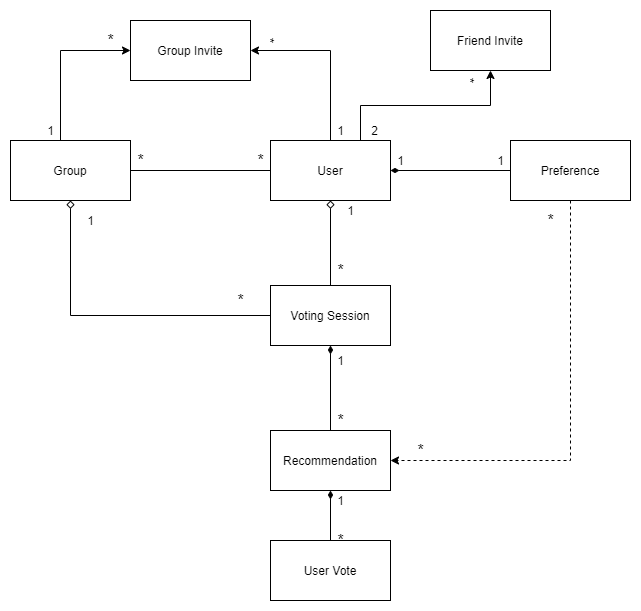
\includegraphics[width=0.7\textwidth]{uml-diagram.png}
	\caption{UML Diagram across data models}
	\label{FigUH}
\end{figure}

\section{Module Hierarchy} \label{SecMH}

This section provides an overview of the module design. Modules are summarized
in a hierarchy decomposed by secrets in Table \ref{TblMH}. The modules listed
below, which are leaves in the hierarchy tree, are the modules that will
actually be implemented.

\begin{description}
\item [\refstepcounter{mnum} \mthemnum \label{mHH}:] Hardware-Hiding Module
\item [\refstepcounter{mnum} \mthemnum \label{mBH}:] Behaviour-Hiding Module
	\begin{itemize}
		\item [\refstepcounter{mnum} \mthemnum \label{mNL}:] Native Login Module
		\item [\refstepcounter{mnum} \mthemnum \label{mF}:] Friends Module
		\item [\refstepcounter{mnum} \mthemnum \label{mG}:] Groups Module
		\item [\refstepcounter{mnum} \mthemnum \label{mP}:] Profile Module
	\end{itemize}
\item [\refstepcounter{mnum} \mthemnum \label{mSD}:] Software Decision Module
	\begin{itemize}
		\item [\refstepcounter{mnum} \mthemnum \label{mMA}:] Matching Algorithm Module
		\item [\refstepcounter{mnum} \mthemnum \label{mOL}:] OAuth Login Module
		\item [\refstepcounter{mnum} \mthemnum \label{mA}:] API Module
	\end{itemize}
\end{description}


\begin{table}[h!]
\centering
\begin{tabular}{p{0.3\textwidth} p{0.6\textwidth}}
\toprule
\textbf{Level 1} & \textbf{Level 2}\\
\midrule

{Hardware-Hiding Module} & ~ \\
\midrule

\multirow{4}{0.3\textwidth}{Behaviour-Hiding Module} & {Native Login Module}\\
& Friends Module\\
& Groups Module\\
& Profile Module\\
\midrule

\multirow{3}{0.3\textwidth}{Software Decision Module} & {Matching Algorithm Module}\\
& OAuth Login Module\\
& API Module\\
\bottomrule

\end{tabular}
\caption{Module Hierarchy}
\label{TblMH}
\end{table}

\section{Connection Between Requirements and Design} \label{SecConnection}

The design of the system is intended to satisfy the requirements developed in
the SRS. In this stage, the system is decomposed into modules. The connection
between requirements and modules is listed in Table~\ref{TblRT}.

\section{Module Decomposition} \label{SecMD}

Modules are decomposed according to the principle of ``information hiding''
proposed by \citet{ParnasEtAl1984}. The \emph{Secrets} field in a module
decomposition is a brief statement of the design decision hidden by the
module. The \emph{Services} field specifies \emph{what} the module will do
without documenting \emph{how} to do it. For each module, a suggestion for the
implementing software is given under the \emph{Implemented By} title. If the
entry is \emph{OS}, this means that the module is provided by the operating
system or by standard programming language libraries.  \emph{\progname{}} means the
module will be implemented by the \progname{} software.

Only the leaf modules in the hierarchy have to be implemented. If a dash
(\emph{--}) is shown, this means that the module is not a leaf and will not have
to be implemented.

\subsection{Hardware Hiding Modules (\mref{mHH})}

\begin{description}
\item[Secrets:]The data structure and algorithm used to implement the virtual
  hardware.
\item[Services:]Serves as a virtual hardware used by the rest of the
  system. This module provides the interface between the hardware and the
  software. So, the system can use it to display outputs or to accept inputs.
\item[Implemented By:] OS
\end{description}

\subsection{Behaviour-Hiding Module (\mref{mBH})}

\begin{description}
\item[Secrets:]The contents of the required behaviours.
\item[Services:]Includes programs that provide externally visible behaviour of
  the system as specified in the software requirements specification (SRS)
  documents. This module serves as a communication layer between the
  hardware-hiding module and the software decision module. The programs in this
  module will need to change if there are changes in the SRS.
\item[Implemented By:] --
\end{description}

%\subsubsection{Input Format Module (\mref{mInput})}
%
%\begin{description}
%\item[Secrets:]The format and structure of the input data.
%\item[Services:]Converts the input data into the data structure used by the
%  input parameters module.
%\item[Implemented By:] [Your Program Name Here]
%\item[Type of Module:] [Record, Library, Abstract Object, or Abstract Data Type]
%  [Information to include for leaf modules in the decomposition by secrets tree.]
%\end{description}

\subsubsection{Native Login Module (\mref{mNL})}

\begin{description}
\item[Secrets:] Hides authentication data from the rest of the software, isolating the authentication as the rest of the software has no use for a user's email or password
\item[Services:] Native log in to the application
\item[Implemented By:] \progname
\item[Type of Module:] Record
\end{description}

\subsubsection{Friends Module (\mref{mF})}

\begin{description}
\item[Secrets:] The methodology and data related to adding/deleting friends
\item[Services:] Allows a user to add and delete friend's but sharing their nickname or email address with one another
\item[Implemented By:] \progname
\item[Type of Module:] Record
\end{description}

\subsubsection{Groups Module (\mref{mG})}

\begin{description}
\item[Secrets:] The methodology and data used to create a group with other friends
\item[Services:] Allows the user to create, join, leave, and delete individual groups, invite friends, and receive recommendations on a show to watch based on the groups' preferences
\item[Implemented By:] \progname
\item[Type of Module:] Abstract Object
\end{description}

\subsubsection{Profile Module (\mref{mP})}

\begin{description}
\item[Secrets:] The methodology and data for an individual user
\item[Services:] Allows the user to modify their preferences and general profile
\item[Implemented By:] \progname
\item[Type of Module:] Abstract Object
\end{description}

\subsection{Software Decision Module (\mref{mSD})}

\begin{description}
\item[Secrets:] The design decision based on mathematical theorems, physical
  facts, or programming considerations. The secrets of this module are
  \emph{not} described in the SRS.
\item[Services:] Includes data structure and algorithms used in the system that
  do not provide direct interaction with the user. 
  % Changes in these modules are more likely to be motivated by a desire to
  % improve performance than by externally imposed changes.
\item[Implemented By:] --
\end{description}

\subsubsection{Matching Algorithm Module (\mref{mMA})}

\begin{description}
\item[Secrets:] The methodology and data on how recommendations are created
\item[Services:] Converts the input data to a list of recommendations for a \verb_group_
\item[Implemented By:] \progname
\item[Type of Module:] Abstract Object
\end{description}

\subsubsection{OAuth Login Module (\mref{mOL})}

\begin{description}
\item[Secrets:] OAuthentication login details, through Google
\item[Services:] Allows the user to sign up and login through an OAuth provider
\item[Implemented By:] Google OAuth services paired with \progname
\item[Type of Module:] Library
\end{description}

\subsubsection{API Module (\mref{mA})}

\begin{description}
\item[Secrets:] Data behind fetching all the shows and organizing them
\item[Services:] Allows \progname ~ to return a set of shows that match user preferences
\item[Implemented By:] OMDb API and Jikan Anime API
\item[Type of Module:] Library
\end{description}

\section{Traceability Matrix} \label{SecTM}

This section shows two traceability matrices: between the modules and the
requirements and between the modules and the anticipated changes.

% the table should use mref, the requirements should be named, use something
% like fref
\begin{table}[H]
\centering
\begin{tabular}{p{0.2\textwidth} p{0.6\textwidth}}
\toprule
\textbf{Req.} & \textbf{Modules}\\
\midrule
R1 & \mref{mNL}\\
R2 & \mref{mOL}\\
R3 & \mref{mNL}, \mref{mOL}\\
R4 & \mref{mP}\\
R5 & \mref{mP}\\
R6 & \mref{mG}\\
R7 & \mref{mF}, \mref{mG}\\
R8 & \mref{mF}\\
R9 & \mref{mG}, \mref{mMA}, \mref{mA}\\
R10 & \mref{mG}, \mref{mP}\\
R11 & \mref{mG}, \mref{mP}\\
\bottomrule
\end{tabular}
\caption{Trace Between Requirements and Modules}
\label{TblRT}
\end{table}

\begin{table}[H]
\centering
\begin{tabular}{p{0.2\textwidth} p{0.6\textwidth}}
\toprule
\textbf{AC} & \textbf{Modules}\\
\midrule
\acref{acHardware} & \mref{mHH}\\
\acref{acPrefs} & \mref{mP}\\
\bottomrule
\end{tabular}
\caption{Trace Between Anticipated Changes and Modules}
\label{TblACT}
\end{table}

\section{Use Hierarchy Between Modules} \label{SecUse}

In this section, the uses hierarchy between modules is
provided. \citet{Parnas1978} said of two programs A and B that A {\em uses} B if
correct execution of B may be necessary for A to complete the task described in
its specification. That is, A {\em uses} B if there exist situations in which
the correct functioning of A depends upon the availability of a correct
implementation of B.  Figure \ref{FigUH} illustrates the use relation between
the modules. It can be seen that the graph is a directed acyclic graph
(DAG). Each level of the hierarchy offers a testable and usable subset of the
system, and modules in the higher level of the hierarchy are essentially simpler
because they use modules from the lower levels.

\begin{figure}[H]
\centering
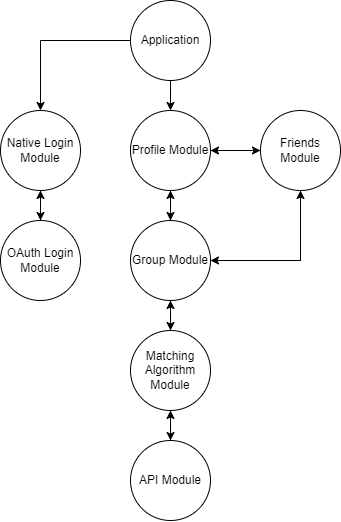
\includegraphics[width=0.7\textwidth]{UsesHierarchy.png}
\caption{Use hierarchy among modules}
\label{FigUH}
\end{figure}

\newpage

%\section*{References}

\bibliographystyle {plainnat}
\bibliography{../../../refs/References}

\end{document}